\section{Anatomical data and initialization}\label{app:data}
The files are \path{data/t1_icbm_normal_1mm_pn0_rf0.nii.gz} and \path{data/phantom_1.0mm_normal_crisp.nii.gz}. The former is the BrainWeb T1 alias with 1 mm spacing, zero added noise and zero intensity nonuniformity; the latter is the matching original normal crisp phantom, converted from MINC to NIfTI. These are not the separate BrainWeb 20-subject anatomical models. Both native arrays have shape $181\times217\times181$ and the same RAS+ affine
\begin{equation}
 A=\begin{pmatrix}1&0&0&-90\\0&1&0&-126\\0&0&1&-72\\0&0&0&1\end{pmatrix}.
\end{equation}
Native gray- and white-matter voxel counts are 902,912 and 674,777. Tissue labels 2, 3 and 8 define the active domain; label 8 uses gray-matter coefficients. CSF is label 1 and is excluded. No tumor is present in the source images. T1 intensities are divided by their 99.8th percentile and clipped for background display only; they do not determine transport or growth coefficients. At 2 mm the affine diagonal is $(2,2,2,1)$ with the same translation, and array shape is $91\times109\times91$.

The SHA-256 checksums of the bundled compressed files are:
\begin{quote}\footnotesize
T1: \nolinkurl{aa40262b2702653188fd51bdec844a393b825650fe1155a84d8606f5dfd99eb3}\\
Labels: \nolinkurl{afdff78fc1b06ad7c7d8216cf96be737a1450ef5b6abf27eb732c0bf8b66fac0}.
\end{quote}
The manifest retains official aliases and source URLs. Regenerating a MINC-to-NIfTI conversion can change compression/header encoding and therefore file hashes; a replacement requires an explicit voxel/affine comparison and updated manifest. BrainWeb attribution and terms remain applicable to these data.

For $\bm{x}_0=(-30,25,30)$ mm and $\sigma_k=6$ mm, let $r^2=\sum_{k=1}^{3}[(x_k-x_{0k})/\sigma_k]^2$. The initialization is
\begin{equation}
 c(\bm{x},0)=80{,}000\exp(-r^2/2)\,\mathbf{1}_{\{r^2\leq9\}}\,\mathbf{1}_{\Omega}(\bm{x}),\qquad z(\bm{x},0)=0 .
\end{equation}
Oxygen is initialized by the elliptic solve. The physical center is retained when grids change. The nearest saved slice indices on the 2 mm grid are $(30,76,51)$, corresponding to RAS $(-30,26,30)$ mm: the saved coronal plane is at 26 mm, rather than the off-grid 25 mm seed coordinate. Figure~\ref{fig:orthogonal} supplies orthogonal views of the same fields as Figure~\ref{fig:fields}.

\begin{figure}[p]
\centering
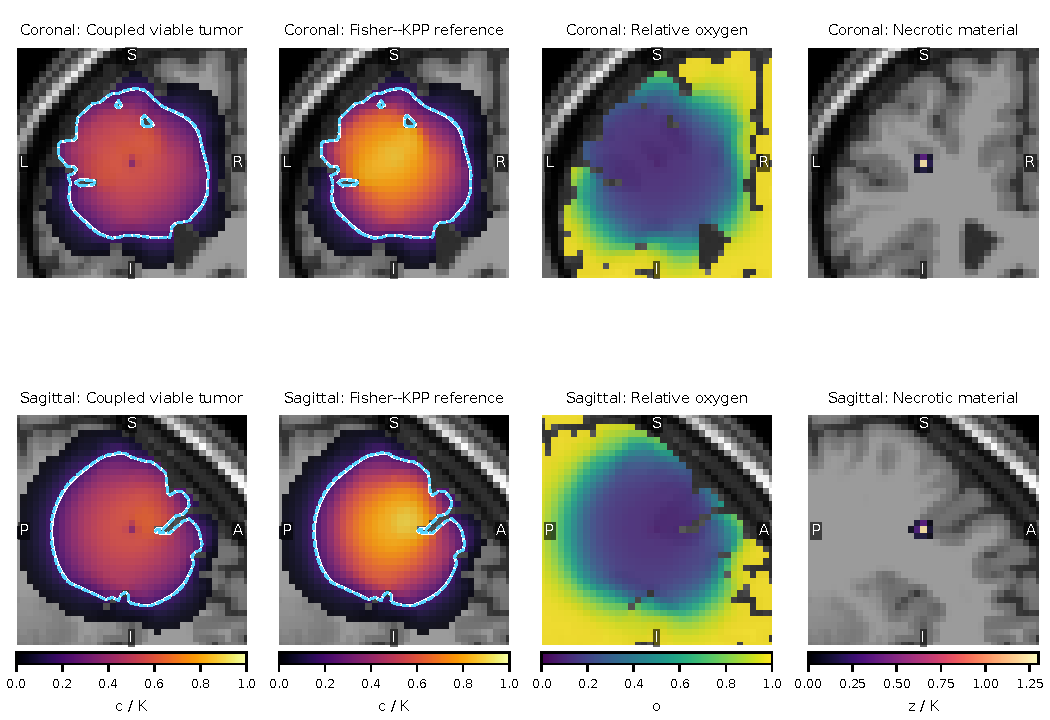
\includegraphics[width=\textwidth]{figures/orthogonal_fields.pdf}
\caption{Orthogonal day-90 comparisons through the saved seed planes: coronal $y=26$ mm (top) and sagittal $x=-30$ mm (bottom). Each panel spans $72\times72$ mm with native 2 mm pixels. Columns show coupled viable density, the matched Fisher--KPP reference, relative oxygen and necrotic material. The viable and reference scales are identical, and the necrotic scale extends to 1.3. White solid and cyan dashed contours indicate the respective $c/K=0.2$ boundaries.}\label{fig:orthogonal}
\end{figure}

\section{Numerical implementation and verification}\label{app:numerics}
\subsection{Conservative transport and reaction splitting}
For neighboring active cells $i,j$ on a Cartesian grid of spacing $h$, use the harmonic face coefficient
\begin{equation}
 D_{ij}=\begin{cases}2D_iD_j/(D_i+D_j),&D_i+D_j>0,\\0,&\text{otherwise},\end{cases}\qquad
 w_{ij}=D_{ij}/h^2 .
\end{equation}
Faces leaving the active domain are assigned zero weight, as are external volume faces. A cell-transport step is
\begin{equation}
 c_i^*=c_i^n+\Delta t\sum_{j\in\mathcal N(i)}w_{ij}(c_j^n-c_i^n),\qquad
 \Delta t\leq\frac{0.9}{\max_i\sum_j w_{ij}} .
\end{equation}
Symmetric fluxes conserve total cell count under pure diffusion. The step bound is sufficient for nonnegative explicit updates. Faces are stored without periodic wrapping; no density clipping is applied. Requested steps are subdivided as needed, and steps end at the exact saved output times.

For M0, the reaction following diffusion is the exact logistic flow
\begin{equation}
 c_i^{n+1}=\frac{c_i^*}{\exp(-\rho_i\Delta t)+(c_i^*/K_i)[1-\exp(-\rho_i\Delta t)]}.
\end{equation}
For M2, freeze oxygen at $o^n$ and necrosis at $z^n$ during birth. Set $F_i=K_i-z_i^n$. If $F_i>0$ and $c_i^*<F_i$, use
\begin{equation}
 r_i=\rho_i g(o_i^n)F_i/K_i,\qquad
 c_i^b=\frac{c_i^*}{\exp(-r_i\Delta t)+(c_i^*/F_i)[1-\exp(-r_i\Delta t)]}.
\end{equation}
Otherwise $c_i^b=c_i^*$. With $q_i=\delta h(o_i^n)$, the subsequent death/clearance step is
\begin{equation}
 L_i=c_i^b[1-\exp(-q_i\Delta t)],\quad
 c_i^{n+1}=c_i^b-L_i,\quad
 z_i^{n+1}=(z_i^n+L_i)\exp(-\lambda_z\Delta t).
\end{equation}
The same $L_i$ leaves $c$ and enters $z$, preserving cell equivalents when clearance is zero. Exact frozen-coefficient substeps do not make the full coupled update exact: diffusion, birth, death and clearance are Lie-split, and oxygen is lagged. The complete method is first order in time. The centered spatial stencil has second-order consistency in smooth regions, without a global spatial-order claim at sharp tissue boundaries. Tumor and necrosis arrays use float32 and compiled Numba CPU kernels.

\subsection{Quasi-steady oxygen solve}
Let $L_h$ be the unit-diffusivity no-flux Laplacian on the active voxel graph, $u=c/K$, and $p_i=[1+\alpha(c_i+z_i)/K_i]^{-1}$. After initialization and each tumor update, solve
\begin{equation}
 \left[-\ell_o^2L_h+\operatorname{diag}(p+\beta u)\right]\bm{o}=\bm{p}.
\end{equation}
The positive reaction diagonal makes this system symmetric positive definite, including disconnected tissue components. Matrix-free conjugate gradients use float64 arithmetic, the previous oxygen state as the initial guess and a Jacobi preconditioner. The relative residual tolerance is $10^{-7}$, with a 200-iteration maximum per solve. Nonconvergence or oxygen-bound failure raises an error. The zero-uptake and zero-diffusion limits have direct solutions. Stored oxygen is float32. Outside-domain zeros are excluded-domain sentinels and are excluded from oxygen statistics and overlays.

The primary M2 run required 361 solves and 873 total conjugate-gradient iterations; the largest recorded relative residual was below $10^{-7}$. This residual measures algebraic solution accuracy, not accuracy of the continuum approximation on the chosen grid.

\subsection{Recorded checks and refinement comparisons}
The \TestCount{}-test suite includes exact logistic growth; reflecting-boundary diffusion modes; heterogeneous-flux conservation; impermeable interfaces and no wrapping; positivity and unsafe-step rejection; parameter checks; exact output times; data affine/tissue checks; uniform and nonuniform oxygen solutions; oxygen barriers; exact death transfer and clearance; occupied-capacity behavior; Fisher--KPP recovery; live-plus-dead balance; coupled temporal refinement against an independent Runge--Kutta calculation; failed-solver reporting; rendering; and replay compatibility. Test results are stored in \texttt{paper/data/pytest.xml}. Notebook smoke checks and media review are separate interface checks.

For field $v$, final relative $L^2$ differences are $\|v_{\Delta t}-v_{0.0625}\|_2/\|v_{0.0625}\|_2$ on the same 2 mm grid (Table~\ref{tab:errors}). The denominator is nonzero in these cases. These are finite-reference differences, not rigorous continuum error bounds. The 1 mm assessment is reported in Table~\ref{tab:refinement}; because the tissue labels also change under resampling, it is not used to infer spatial order.

\begin{table}[tbp]
\centering\small
\caption{Final relative $L^2$ differences (percent) against the 0.0625-day M2 calculation on the 2 mm grid.}\label{tab:errors}
\begin{tabular}{rrrr}
\toprule $\Delta t$ (days) & Viable tumor & Oxygen & Necrotic material\\\midrule
\ErrorRows
\bottomrule
\end{tabular}
\end{table}

\section{Inverse formulation, priors and identifiability}\label{app:inference}
\subsection{An example estimation objective}
With the observation model in Equation~\eqref{eq:observation}, a possible maximum-a-posteriori objective for continuous approximately Gaussian observations is
\begin{align}
 (\widehat{\bm\theta},\widehat{\bm\eta})
 &=\arg\min_{\bm\theta,\bm\eta}\ \mathcal J(\bm\theta,\bm\eta),\\
 \mathcal J&=\frac12\sum_{m,j}\bm r_{mj}^{\mathsf T}\Sigma_{mj}^{-1}\bm r_{mj}
 -\log\pi(\bm\theta,\bm\eta),\qquad
 \bm r_{mj}=\mathcal H_m[\bm s_{\bm\theta}(t_j);\bm\eta_m]-\bm y_{mj},
\end{align}
where $\bm s=(c,o,z)$ and $\Sigma$ models measurement covariance. Cross-time or cross-modality correlations require a joint likelihood rather than independent terms. Segmentations may need a probabilistic classification likelihood rather than Gaussian residuals. Registration, partial volume, scanner bias, initial fields and uncertain state-to-signal mappings should enter the likelihood or be propagated as nuisance uncertainty. Bayesian sampling can quantify uncertainty; an optimizer alone does not provide calibrated predictive intervals. No such fit was performed in this study.

\subsection{Important structural and practical ambiguities}
\begin{enumerate}
\item \textbf{Absolute cell scale.} In terms of $u=c/K$ and $w=z/K$ with uniform $K$, the normalized dynamics do not determine $K$. Scaling $(c,z,K)$ together leaves $(u,w,o)$ unchanged. An observation dependent only on normalized density cannot identify the absolute cell count without external calibration.
\item \textbf{Age and rates.} For an unknown elapsed tumor age, multiplying $D$, $\rho$, $\delta$ and $\lambda_z$ by a common factor and dividing the elapsed time by that factor leaves the autonomous state trajectory at the observation unchanged. Known longitudinal time intervals can break this particular scaling, although seed and parameter confounding may remain.
\item \textbf{Oxygen-growth coupling.} Where all observed cells remain below $\theta_p$, the birth term depends on $\rho/\theta_p$ rather than on those parameters separately, for a fixed oxygen field. Oxygen threshold calibration and observations spanning informative regimes are needed.
\item \textbf{Delivery and uptake.} Neglecting spatial oxygen transport locally gives
\begin{equation}
 o=\frac{1}{1+\beta u[1+\alpha(u+w)]}.
\end{equation}
One local state constrains an effective supply--uptake combination, not separate mechanisms. Spatially varying, calibrated oxygen observations across burdens could help, but do not guarantee recovery. An exchange length far below measurement and mesh resolution can be practically unidentifiable.
\item \textbf{Quasi-steady reduction.} If a dimensional oxygen equation is divided by a baseline restoration rate, $\ell_o^2$ and $\beta$ represent coefficient ratios. Steady observations alone cannot identify an independent absolute oxygen relaxation time removed by that reduction.
\item \textbf{Necrotic history.} For known $q=\delta h(o)$,
\begin{equation}
 z(t)=z(0)e^{-\lambda_z t}+\int_0^t q(s)c(s)e^{-\lambda_z(t-s)}\,\dd s .
\end{equation}
A single terminal necrotic measurement cannot generally separate formation history and clearance. Zero clearance is a model choice here, not an estimated absence of biological removal.
\end{enumerate}

Positive parameters can be transformed as $\log\theta_k\sim\mathcal N(\mu_k,\sigma_k^2)$, with dimensional reference units stated. For thresholds, use $\theta_p=\operatorname{logit}^{-1}(a)$ and $\theta_d=\theta_p\operatorname{logit}^{-1}(b)$. A zero-clearance component or other exact-zero ablation requires an explicit point mass or a separate model, rather than a continuous positive prior. Neither prior hyperparameters nor population distributions are supplied by the current phantom experiment.

Before a full fit, evaluate scaled observation sensitivities, their singular values, profile likelihoods and posterior dependence across plausible initial states and observation mappings. The number of voxels is not the number of independent constraints. Begin with a global migration scale and growth coefficient, restrict other quantities using external information, and add freedom only when independent observations support it. Identifiability and predictive comparison should be repeated for each candidate model and intended measurement set.

\section{Reproducibility and interactive artifacts}
\path{paper/run_experiments.py} runs the nine model/step/grid cases using \path{examples/coupled.json}, verifies the bundled data and checks that the primary viable-count trajectory matches the saved example. It records final metrics and settings in \texttt{experiments.json}, time courses in \texttt{timecourses.csv}, lossless final seed-plane fields in \texttt{day90\_planes.npz}, and provenance in \texttt{provenance.json}, all under \texttt{paper/data/}. Source hashes include the model, data loader, renderer, configuration, lockfile and experiment script. The experiments were generated before their implementation changes were committed, so provenance records working-file hashes alongside the base Git revision. The hashes identify the simulation sources independently of that earlier revision.

\texttt{paper/make\_figures.py} reads these records to generate figures, table rows and numerical macros used directly by the manuscript. The local Python environment is defined by \texttt{pyproject.toml} and \texttt{uv.lock}. A \texttt{Makefile} rebuilds the figures and PDF, with a separate target to rerun the experiments. The native and 2 mm examples are deterministic; they do not sample biological uncertainty.

\texttt{tumor\_growth\_explorer.ipynb} exposes both models; \texttt{coupled\_example.ipynb} presets the 90-day comparison. Time and RAS slices are shared across the four-field view. Live histories permit arbitrary 3D slicing, while compact replay files retain the three seed-plane histories and final full volumes. The slower comparison MP4 uses 400 frames at 20 frames/s, including a 120-frame day-90 hold; playback duration is distinct from simulated time. Synchronized movies help inspect output but are not quantitative validation. Manuscript figures retain the full computed necrotic range, unlike a display limited to $0$--$1$.
